\section{Methods}\label{section:methods}
\kant[5]

\subsection{Technique 1}
\kant[6]

% =======================================================
\begin{equation}\label{eq:entropy}
S=-k_{\textrm{B}}\sum_{i}\rho_{i}\ln\rho_{i}
\end{equation}
% =======================================================

\kant[7]

% =======================================================
\begin{figure}[h]\label{fig:test_inset}
\begin{center}
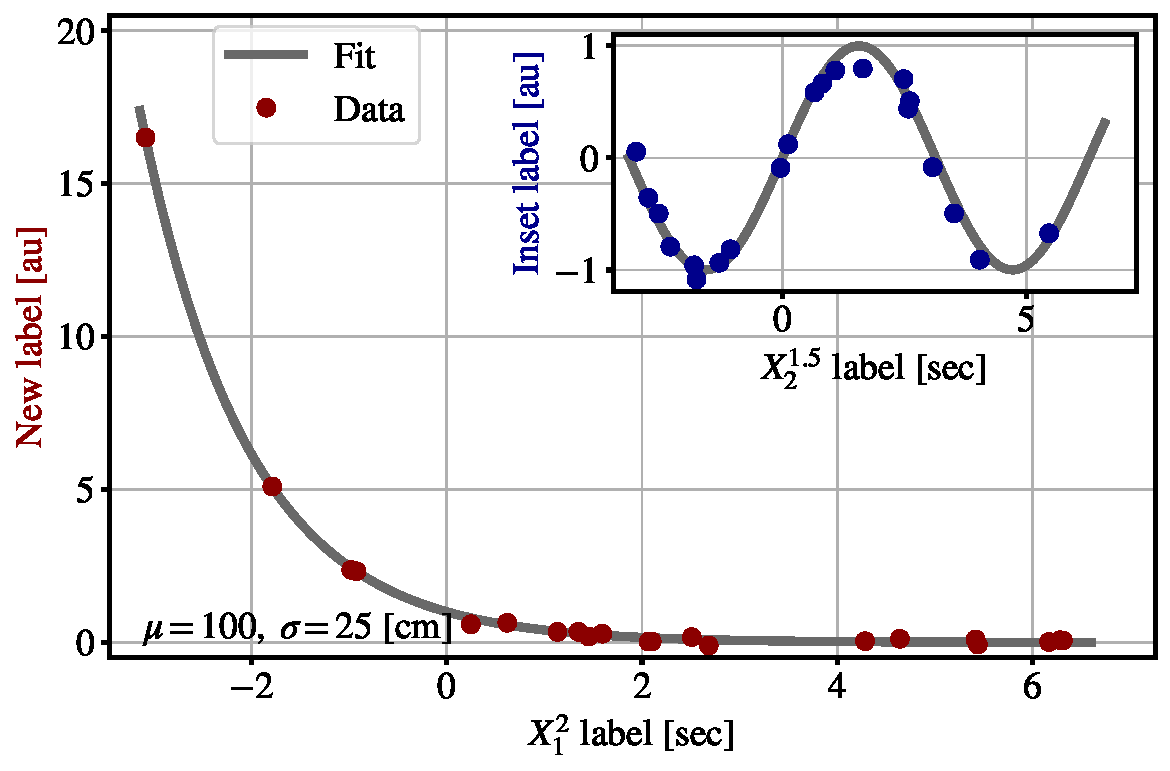
\includegraphics[scale=0.6]{figures/test_inset.pdf}
\end{center}
\caption{This is a test figure with an inset.}
\end{figure}
% =======================================================

\kant[8] And there's more to be written about this topic.~\cite{einstein}

% =======================================================
\begin{table}[h]\label{tab:zoo_animal_prices}
\begin{center}\begin{tabular}{llr}
\toprule
\multicolumn{2}{c}{Item} \\
\cmidrule(r){1-2}
Animal    & Description & Price (\$) \\
\midrule
Gnat      & per gram    & 13.65      \\
          &    each     & 0.01       \\
Gnu       & stuffed     & 92.50      \\
Emu       & stuffed     & 33.33      \\
Armadillo & frozen      & 8.99       \\
\bottomrule
\end{tabular}\end{center}
\caption{Example of current zoo animal prices.}
\end{table}
% =======================================================

\kant[9]
